\documentclass[11pt,a4paper]{article}
\usepackage[a4paper,margin=2cm]{geometry}
\usepackage[T1]{fontenc}
\usepackage{lmodern}
\usepackage{microtype}
\usepackage{booktabs}
\usepackage{tabularx}
\usepackage{enumitem}
\usepackage{xcolor}
\usepackage{tikz}
\usetikzlibrary{positioning,arrows.meta,fit,backgrounds}
\usepackage[hidelinks]{hyperref}

\definecolor{ink}{HTML}{1F2937}
\definecolor{accent}{HTML}{1F6FB2}
\definecolor{soft}{HTML}{E8F1FA}
\definecolor{warn}{HTML}{B45309}
\setlist{nosep,leftmargin=1.2em}
\setlength{\parskip}{0.35em}
\setlength{\parindent}{0pt}

\title{\textbf{Image-to-Cash}\\[0.2em]\large Architecture and design rationale for automating Fakturama from an order image}
\author{Marwan Abdellah}
\date{November 2026}

\begin{document}
\maketitle
\vspace{-1.5em}

\begin{abstract}
\noindent Image-to-Cash turns a single order image (or PDF) into a saved, verified \emph{Order} and a linked, paid
\emph{Invoice} in the Fakturama~2.2.0 desktop application. It drives the real user interface through Microsoft
UI Automation (UIA) and OCR, without stored coordinates, and checks every step against Fakturama's own database. This note
explains the architecture, the principles behind it, and how the design was hardened by the Elephant--Goldfish review
method (EGM) and by live calibration. Source: \url{https://github.com/MarwanAbdellah/TJM-Fakturama-Automation}.
\end{abstract}

\section{The task and its constraints}
The brief asks for ``one continuous Order-first flow'': extract the order, open a \emph{New Order}, use the Order's own
Debtor and Product selectors as the existence checks, create missing master data only when an exact selection is
unavailable, return to the same open Order, complete it, create the linked Invoice from the Order's follow-up area, apply
the payment status, and verify the saved records---``without relying on hardcoded coordinates or a fixed UI layout'',
using UIA, OCR and/or LLMs. Four constraints shaped everything that follows:
\begin{enumerate}
  \item \textbf{The UI is the only write path.} Fakturama is an Eclipse RCP/SWT application; its item table is a NatTable
        that UIA cannot read cell by cell.
  \item \textbf{Every step must be verified} before moving on (brief~\S1--\S5), including the persisted payment state.
  \item \textbf{Wrong data is worse than no data.} A duplicate Debtor or a mispriced line costs more than a stopped run.
  \item \textbf{The flow is fixed by the brief.} A faster ``masters-first'' redesign (pre-create all products, then fill the
        Order) was drafted and reviewed, then deliberately dropped to keep the brief's Order-first semantics.
\end{enumerate}

\section{Architecture}
The system is a pipeline with one data contract, \texttt{OrderDraft} (a Pydantic model), between reading and acting
(Figure~\ref{fig:arch}). Reading never touches Fakturama; acting never re-reads the image.

\begin{figure}[h]
\centering
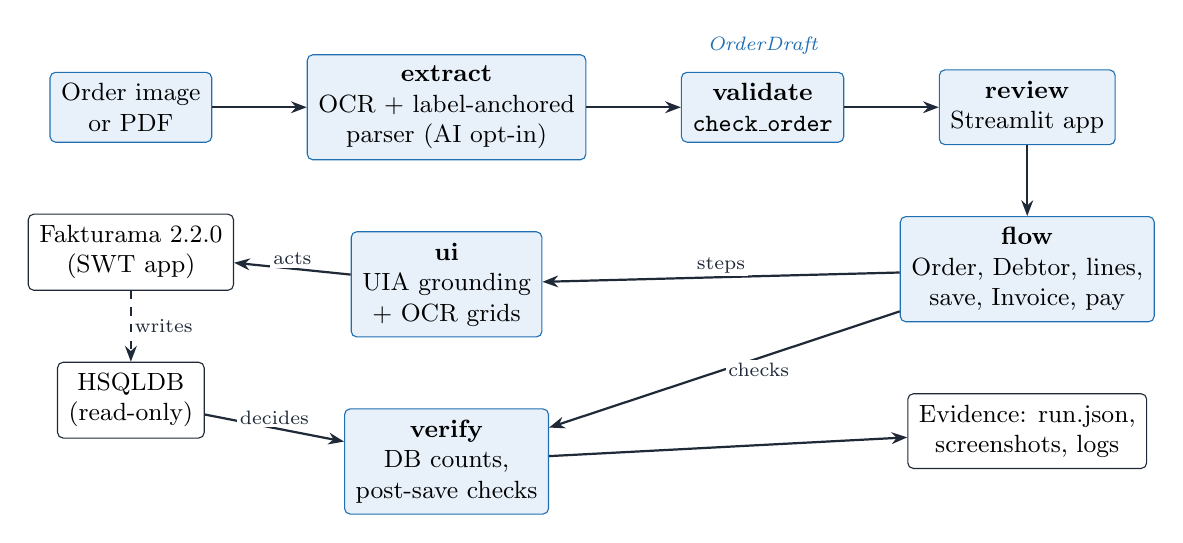
\begin{tikzpicture}[
  box/.style={draw=accent,fill=soft,rounded corners=2pt,align=center,font=\small,minimum height=2.2em,inner sep=4pt},
  db/.style={draw=ink,fill=white,rounded corners=2pt,align=center,font=\small,minimum height=2.2em,inner sep=4pt},
  arr/.style={-{Stealth[length=2mm]},thick,color=ink},
  lbl/.style={font=\scriptsize,color=ink,fill=white,inner sep=1pt},
  node distance=9mm and 12mm]
  % row 1: reading (never touches Fakturama)
  \node[box] (img) {Order image\\ or PDF};
  \node[box,right=of img] (ext) {\textbf{extract}\\ OCR + label-anchored\\ parser (AI opt-in)};
  \node[box,right=of ext] (val) {\textbf{validate}\\ \texttt{check\_order}};
  \node[box,right=of val] (rev) {\textbf{review}\\ Streamlit app};
  % row 2: acting
  \node[box,below=of rev] (flow) {\textbf{flow}\\ Order, Debtor, lines,\\ save, Invoice, pay};
  \node[box,below=of ext] (ui) {\textbf{ui}\\ UIA grounding\\ + OCR grids};
  \node[db,below=of img] (fk) {Fakturama 2.2.0\\ (SWT app)};
  % row 3: deciding and verifying
  \node[db,below=of fk] (hs) {HSQLDB\\ (read-only)};
  \node[box,below=of ui] (ver) {\textbf{verify}\\ DB counts,\\ post-save checks};
  \node[db,below=of flow] (ev) {Evidence: run.json,\\ screenshots, logs};
  \draw[arr] (img) -- (ext);
  \draw[arr] (ext) -- (val);
  \draw[arr] (val) -- (rev);
  \draw[arr] (rev) -- (flow);
  \draw[arr] (flow) -- node[lbl,above]{steps} (ui);
  \draw[arr] (ui) -- node[lbl,above]{acts} (fk);
  \draw[arr,dashed] (fk) -- node[lbl,right]{writes} (hs);
  \draw[arr] (hs) -- node[lbl,above]{decides} (ver);
  \draw[arr] (flow) -- node[lbl,right]{checks} (ver);
  \draw[arr] (ver) -- (ev);
  \node[font=\scriptsize\itshape,color=accent,above=1mm of val.north] {OrderDraft};
\end{tikzpicture}
\caption{Pipeline. Reading (top) never touches Fakturama; the UI layer acts; the read-only database decides and
verifies; every run leaves an evidence trail. \texttt{OrderDraft} is the one contract between reading and acting.}
\label{fig:arch}
\end{figure}

\begin{description}[leftmargin=0pt,style=nextline]
  \item[Extraction.] A local OCR engine (Indra) feeds a parser that anchors on printed labels rather than positions, so the
        template survives shifts and rescans. For layouts it cannot read, an \emph{opt-in} and still \emph{experimental} vision model (any
        OpenAI-compatible endpoint; OpenRouter by default) fills the same schema. It is off by default because the image
        leaves the machine; its output gets no special trust: the same checks, a second reading told exactly which checks
        failed, and human review.
  \item[Control grounding.] Controls are found by a ladder, cheapest and most stable first: (1)~the UIA name (toolbar
        tooltips, navigation links, totals); (2)~a \emph{label anchor}, the nearest field right of or below a static label;
        (3)~a combo identified by the options it offers; (4)~OCR of the NatTable grid, with columns taken from the
        \emph{drawn} grid lines and named by a majority vote of the readable headers.
  \item[Decision and verification.] Fakturama's HSQLDB is opened strictly read-only over JDBC. It answers the questions
        OCR must not: ``does this SKU exist exactly once?'', ``was the Debtor saved with both address roles?'', ``is the
        Invoice linked to this Order, paid, with this date and value?''
  \item[Operation.] A Streamlit app reviews drafts, previews what will be selected or created, books single orders or a
        batch, and pages through each run's steps and screenshots. A CLI does the same headless.
\end{description}

\section{The mind behind it: design principles}
\begin{tabularx}{\linewidth}{@{}>{\raggedright\arraybackslash\bfseries}p{3.9cm}X@{}}
\toprule
Principle & What it means in the code \\
\midrule
OCR locates, the DB decides & An ``exact match'' is a database count: 0 $\Rightarrow$ create, 1 $\Rightarrow$ select,
  $\ge$2 $\Rightarrow$ stop. A grid row that looks right but is not confirmed by the DB stops the run. \\
Stop, don't guess & Two failure types: \texttt{ManualReview} (the data is ambiguous; a human decides) and
  \texttt{AutomationError} (the UI did not reach the expected state). Neither is retried silently. \\
Read back every write & Every typed value is read back; every line is confirmed by the running \emph{Total Net}; every
  save is confirmed by a new database row. \\
Prices come from the catalogue & Product prices are never typed into the Order; a catalogue price that differs from the
  order stops the run instead of being overwritten. \\
Idempotent and resumable & A reference that already has documents is never booked twice; a saved Order without an
  Invoice resumes at the Invoice step after being re-verified against the image. \\
Safe by construction & The test Fakturama is driven if open, otherwise the single open one; either way it must own the
  database port, so checks never read another instance's data. One run
  at a time (file lock), never close an unsaved tab, no machine-specific paths in code. \\
\bottomrule
\end{tabularx}

\section{How the design was hardened}
\paragraph{Elephant--Goldfish Method (EGM).} Each design was reviewed with EGM: the \emph{elephant} (the drafting agent,
with full context: brief, prototype, live UIA probes) writes the design; \emph{goldfish} reviewers with zero context
(design critic, comprehension, implementation readiness, code details, zoom-out/simplicity) read only the artefacts, and a
synthesizer merges, de-duplicates and re-checks their findings. Every finding is explicitly accepted, adapted or rejected,
and every UI mechanic a reviewer called unproven is spiked against the live application before it is built.
\begin{itemize}
  \item \textbf{Design round:} 14 findings (7 high, 5 medium, 2 low). Examples: ``exact match decided by OCR on truncated
        cells'' $\Rightarrow$ the DB-count rule above; ``SWT date fields ignore plain text'' $\Rightarrow$ a segmented
        date-field driver; ``payment branch under-specified'' $\Rightarrow$ the method is ensured \emph{before} New Debtor,
        because the Debtor editor only loads its payment list when it opens.
  \item \textbf{Whole-repository round (v4):} 5 high, 23 medium, 31 low. The most important high finding (B-H1): the saved
        documents were never checked against the debtor actually chosen. It was fixed by recording the chosen contact and
        asserting it on every receiver row of the saved Order and Invoice; all five high findings were closed.
\end{itemize}

\paragraph{What only the live application revealed.} No reviewer predicted these; calibration runs did. Saving while the
dynamic \emph{Delivery address} tab is active throws a NullPointerException (also visible in the brief's own figures), so
the Invoice-address tab is selected before every save. Selectors auto-accept as soon as one row remains, so search terms
are pasted whole. The VAT field parses ``.'' while price fields follow the locale (``6,25'' became 625\,\%). Fakturama
raises its own \emph{Duplicate Contact} dialog on same name and street, so that rule is now checked in the database first.
OCR can join a right-aligned quantity to the adjacent SKU, which is repaired before lines are compared.

\paragraph{Evidence of quality.} 144 unit tests cover the business rules and the decision points (select-or-create,
post-save checks, batch policy, AI-fallback retries) with the UI and database stubbed; the pre-push hook runs them and
\texttt{ruff}. Live runs on the test workspace booked the template orders end to end and produced a step log and
annotated screenshots for each run. Measurement drove optimisation: an 8-line order spent about 120\,s of 264\,s on
repeated grid OCR, which led to one grid read per line and column-wise filling.

\section{Limits and next steps}
\begin{itemize}
  \item Batch mode retries a stopped order once, skips orders already booked, and pauses on Esc; a stopped run leaves
        its unsaved Order tab for a human.
  \item Only page~1 of a PDF is read; order-level discount and shipping are not mapped; foreign-currency orders stop.
  \item OCR of very long, scrolling item tables is the slowest and least certain step.
\end{itemize}

\paragraph{With three more hours.} The first priority would be to make the AI service more robust. Today it is an
opt-in fallback for layouts the local parser cannot read: one structured-output call to an OpenAI-compatible model
(OpenRouter by default), retried on busy replies and asked once more with the problems the checks found. To trust it
more: run it on every order and compare it field by field with the local OCR, flagging disagreements for review;
measure it on a labelled set of unseen layouts before relying on it; let it fall back to a local vision model when the
service is unavailable, so images can stay on the machine; and keep its answers in the run evidence.

The second would be a reproducible environment, so anyone gets the same setup with one command. Docker fits the parts
that need no screen: OCR, parsing, the checks, the AI reader and the unit tests, pinned in an image with the OCR models
baked in. Docker cannot drive Fakturama itself, because UI Automation needs a real, unlocked Windows desktop session,
which a container does not have. For the end-to-end runs that means a scripted Windows virtual machine (or a Windows
Sandbox configuration) with Fakturama, a test workspace already set to EUR and this repository installed, restored to
the same clean state before every run. After that: a generic watcher for unexpected dialogs, cleanup of a failed run's
records, and running a whole queue in one process.

\end{document}
